\section{Introduction}
\subsection{Équipe}
\begin{frame}
    \frametitle{\color{white}Présentation de l'équipe}
  \begin{center}
    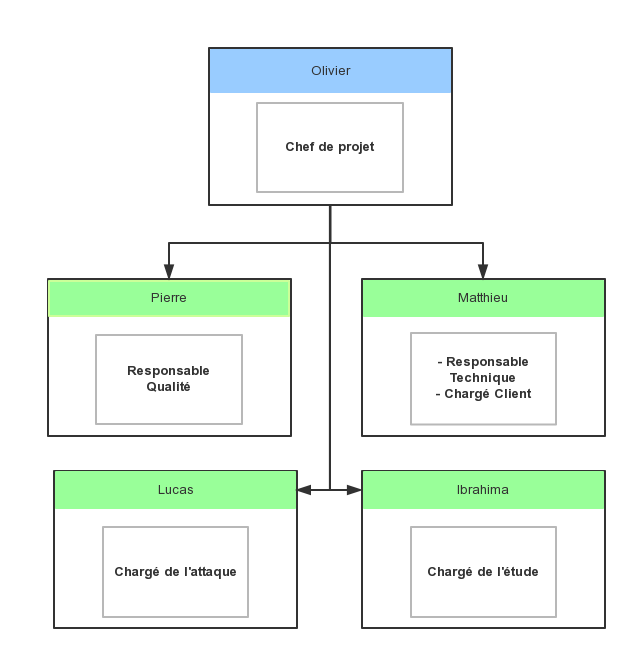
\includegraphics[scale=0.30]{guipgteam.png}
  \end{center}
\end{frame}
\subsection{Organisation}
\begin{frame}
    \frametitle{\color{white}Organisation}
  \begin{block}{Organisation}
    \begin{itemize}
     \item Période : du 20 janvier au 1er mai 2015.
     \item Méthode agile Scrum :
     \begin{itemize}
       \item 2 Sprints.
       \item Réunion quotidienne entre équipiers.
       \item Réunion hebdomadaire avec la cliente.
      \end{itemize}
     \item Gestion du code sur dépôt Git.
     \item Communication :
      \begin{itemize}
       \item Sur Slack entre équipiers.
       \item Par mail via une liste de diffusion avec la cliente.
      \end{itemize}

    \end{itemize}
  \end{block}
\end{frame}